\documentclass{standalone}
\usepackage{pgfplots}
\pgfplotsset{compat=newest}

\begin{document}
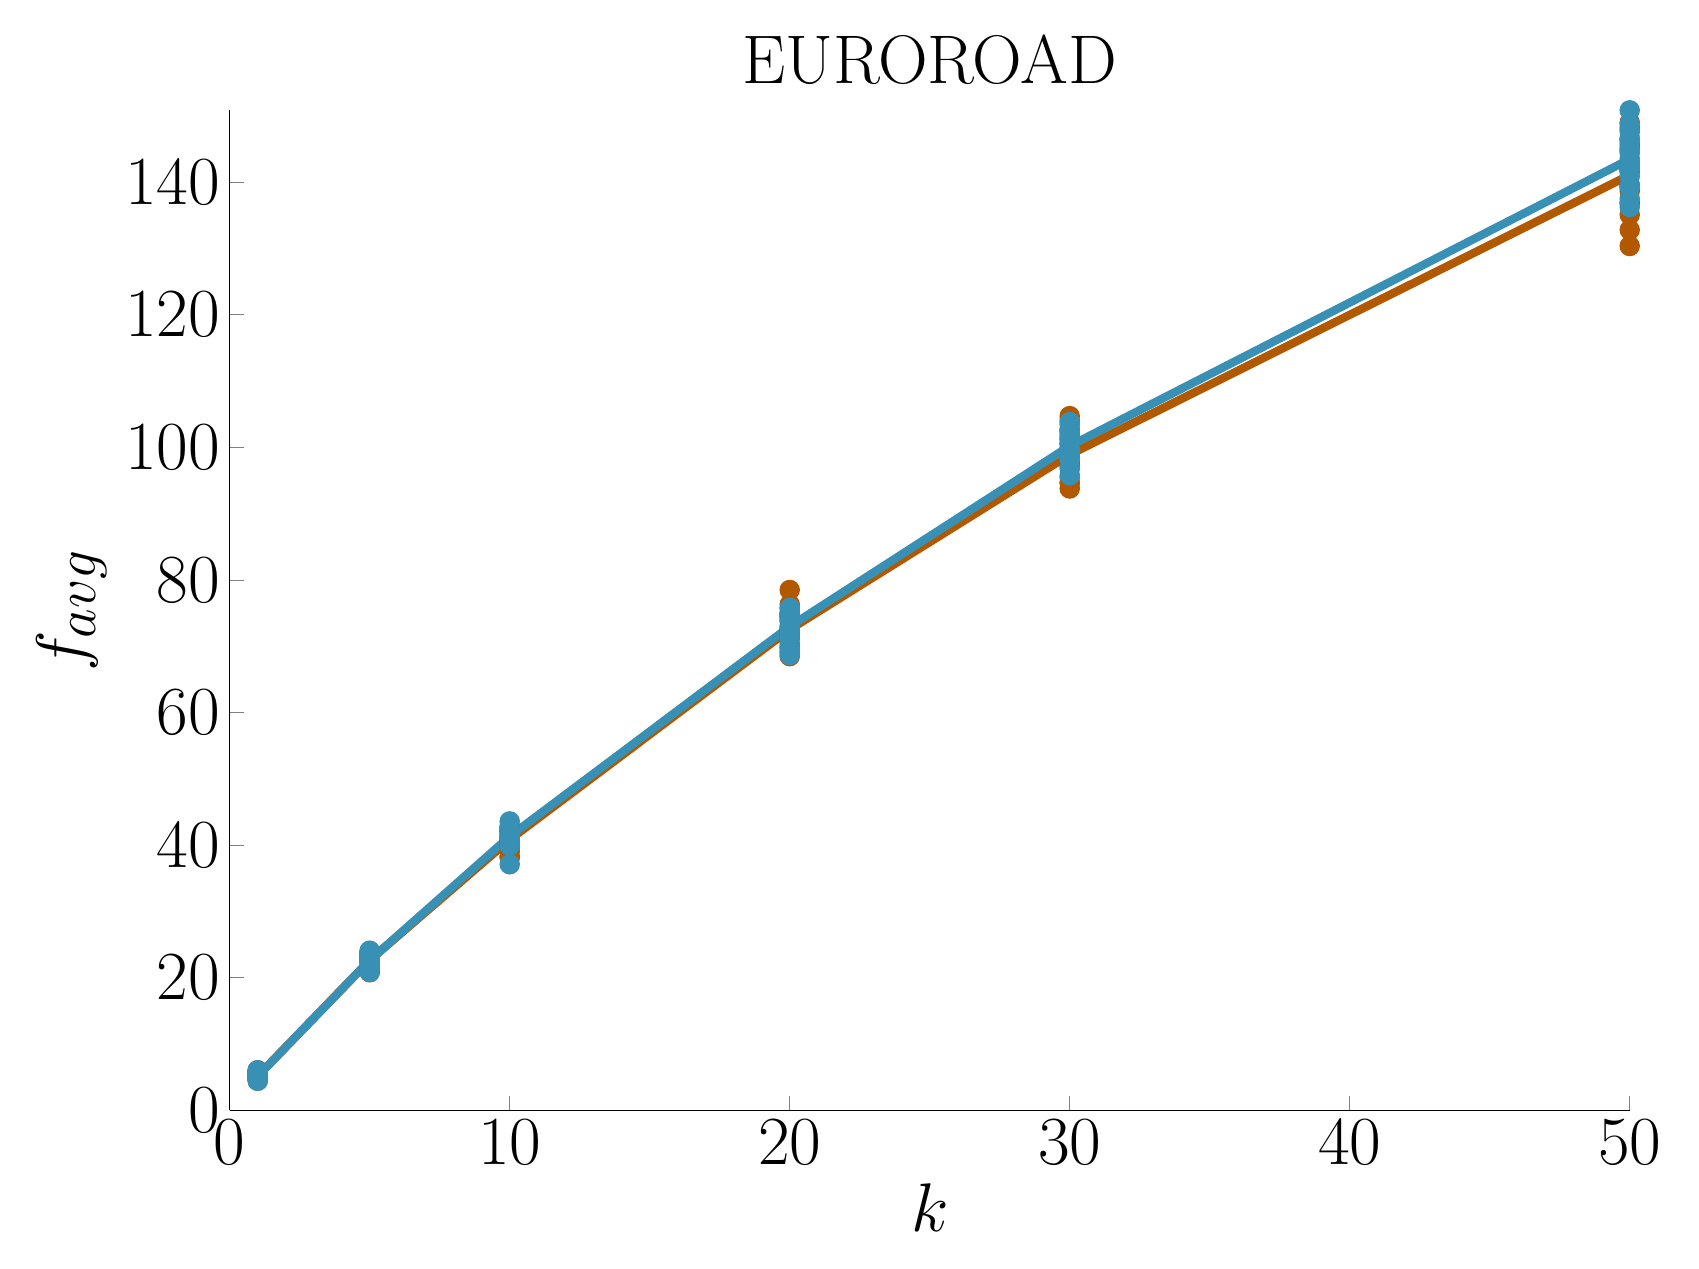
\begin{tikzpicture}

\begin{axis}[%
title style={font=\Huge},
title=EUROROAD,
tick label style={font=\Huge},
label style={font=\Huge},
legend style={font=\Huge},
view={0}{90},
max space between ticks=50pt,
width=7in,
height=5in,
scale only axis,
xmin=0, xmax=50,
xtick={0, 10, 20, 30, 40, 50},
xlabel={$k$},
ymin=0, ymax=150.84,
%ytick={0, 200, 400, 600, 800, 1000},
ylabel={$f_{avg}$},
major tick length=5pt,
axis lines*=left,
legend cell align=left,
clip=false]

\addplot [
only marks,
mark=*,
mark size=3.5pt,
color=orange!70!black,
%solid,
%line width=2pt,
]
coordinates{
(1,4.46)(1,4.78)(1,4.79)(1,4.8)(1,4.81)(1,4.83)(1,4.85)(1,4.94)(1,4.95)(1,5.03)(1,5.06)(1,5.06)(1,5.1)(1,5.26)(1,5.41)(1,5.6)(1,5.63)(1,5.84)(1,5.94)(1,6.04)(5,20.82)(5,21.23)(5,21.27)(5,21.27)(5,22.21)(5,22.31)(5,22.36)(5,22.47)(5,22.59)(5,22.67)(5,22.81)(5,22.86)(5,22.87)(5,23.22)(5,23.4)(5,23.46)(5,23.47)(5,23.52)(5,23.85)(5,23.94)(10,38.12)(10,38.3)(10,39.04)(10,39.56)(10,40.16)(10,40.27)(10,40.33)(10,40.33)(10,40.47)(10,41.08)(10,41.11)(10,41.17)(10,41.23)(10,41.44)(10,41.86)(10,42.15)(10,42.19)(10,42.31)(10,42.61)(10,42.89)(20,68.5)(20,69.14)(20,69.77)(20,69.99)(20,71.17)(20,71.32)(20,71.82)(20,71.83)(20,71.94)(20,72.12)(20,72.25)(20,72.32)(20,72.36)(20,72.45)(20,74.42)(20,74.43)(20,74.87)(20,74.9)(20,76.29)(20,78.49)(30,93.79)(30,94.62)(30,94.62)(30,95.47)(30,97.1)(30,97.51)(30,97.55)(30,98.09)(30,98.2)(30,98.26)(30,98.26)(30,98.53)(30,99.91)(30,100.4)(30,100.57)(30,101.32)(30,102.24)(30,102.54)(30,104.14)(30,104.71)(50,130.37)(50,132.8)(50,135.08)(50,136.86)(50,136.9)(50,138.68)(50,139.15)(50,139.43)(50,139.57)(50,141.61)(50,141.66)(50,141.92)(50,142.0)(50,143.03)(50,145.18)(50,145.67)(50,146.47)(50,147.89)(50,148.26)(50,149.01)
};

\addplot [
only marks,
mark=*,
mark size=3.5pt,
color=cyan!70!black,
%solid,
%line width=2pt,
]
coordinates{
(1,4.46)(1,4.78)(1,4.79)(1,4.8)(1,4.81)(1,4.83)(1,4.85)(1,4.94)(1,4.95)(1,5.03)(1,5.06)(1,5.06)(1,5.1)(1,5.26)(1,5.41)(1,5.6)(1,5.63)(1,5.84)(1,5.94)(1,6.04)(5,20.89)(5,21.05)(5,21.25)(5,21.32)(5,22.11)(5,22.25)(5,22.45)(5,22.5)(5,22.59)(5,22.6)(5,22.66)(5,22.89)(5,22.96)(5,23.28)(5,23.35)(5,23.42)(5,23.46)(5,23.53)(5,23.89)(5,24.08)(10,37.11)(10,39.96)(10,39.97)(10,40.41)(10,40.87)(10,40.98)(10,41.18)(10,41.18)(10,41.34)(10,41.34)(10,41.34)(10,41.37)(10,41.45)(10,42.09)(10,42.1)(10,42.32)(10,42.53)(10,42.55)(10,42.57)(10,43.58)(20,68.68)(20,69.12)(20,69.7)(20,70.46)(20,71.41)(20,72.11)(20,72.23)(20,72.73)(20,72.87)(20,73.05)(20,73.69)(20,73.96)(20,73.97)(20,74.59)(20,74.59)(20,74.83)(20,74.95)(20,75.0)(20,75.74)(20,75.78)(30,95.79)(30,96.8)(30,98.23)(30,98.32)(30,98.55)(30,98.8)(30,99.12)(30,99.17)(30,99.32)(30,99.44)(30,99.87)(30,100.78)(30,101.2)(30,101.68)(30,101.87)(30,102.47)(30,102.6)(30,102.81)(30,103.44)(30,103.83)(50,136.24)(50,137.49)(50,139.32)(50,139.39)(50,140.91)(50,141.86)(50,142.08)(50,142.64)(50,142.65)(50,142.91)(50,143.52)(50,144.45)(50,144.73)(50,144.85)(50,146.12)(50,146.47)(50,146.59)(50,147.61)(50,148.78)(50,150.84)
};

\addplot [
color=orange!70!black,
solid,
line width=3pt
]
coordinates{
(1,5.159)(5,22.63)(10,40.831)(20,72.519)(30,98.8915)(50,141.077)
};

\addplot [
color=cyan!70!black,
solid,
line width=3pt
]
coordinates{
(1,5.159)(5,22.6265)(10,41.312)(20,72.973)(30,100.2045)(50,143.4725)
};


\end{axis}
\end{tikzpicture}
\end{document}
